%
%   This program is free software: you can redistribute it and/or modify
%   it under the terms of the GNU General Public License as published by
%   the Free Software Foundation, either version 3 of the License, or
%   (at your option) any later version.
%
%   This program is distributed in the hope that it will be useful,
%   but WITHOUT ANY WARRANTY; without even the implied warranty of
%   MERCHANTABILITY or FITNESS FOR A PARTICULAR PURPOSE.  See the
%   GNU General Public License for more details.
%
%   You should have received a copy of the GNU General Public License
%   along with this program.  If not, see <http://www.gnu.org/licenses/>.
%

% Version: $Revision: 10671 $

\documentclass[a4paper]{article}

\usepackage{epsfig}
\usepackage{wrapfig}
\usepackage{graphicx}
\usepackage{hyperref}

\title{\epsfig{file=figures/IUB.eps,width=10cm}\vspace{3cm}\\EAR4 Manual\\for Version 1.0}
\author{Vahid Jalali\\David Leake}

\setcounter{secnumdepth}{3}
\setcounter{tocdepth}{3}

\begin{document}

\begin{titlepage}
\maketitle

\thispagestyle{empty}
\center
\begin{table}[b]
\copyright 2014 \\
 \\
Indiana University, Bloomington, Indiana \\
\\
This manual is licensed under the GNU General Public License version 3. More information about this license 
can be found at \url{http://www.gnu.org/licenses/gpl-3.0-standalone.html}
\end{table}

\end{titlepage}

%\tableofcontents

%%%%%%%%%%%%%%%%%%%%%%%%%%%%%%%%%%%
\section{What is EAR4?}
EAR4 is a lazy learner introduced by Jalali and Leake \cite{jalali-Leake13-2}. It applies the
Case-Based Reasoning \cite{mantaras-et-al05} paradigm to regression (i.e. numerical prediction) tasks.
The main idea of EAR4 is very similar to that of IBk \cite{aha91}. 
However, instead of directly using the solutions of the top k nearest neighbors to predict the value
of the input query, EAR4 adjusts the nearest neighbors' values before using them in building 
the solution. Fig. \ref{fig:cbr} depicts the generic process of Case-Based Regression.

\begin{figure}[htb]
  \begin{center}
  \includegraphics[scale=0.5]{figures/cbr.eps}
  \caption{Illustration of the generic case-based regression process}
  \label{fig:cbr}
  \end{center}
\end{figure}

As it can be seen, Case-Based Regression first adjusts the values of the retrieved cases and 
then combines the adjusted values to build the final estimation.

EAR4 utilizes an Ensemble of adaptation rules for adjusting the values of the nearest
neibhbors (also referred to as base cases). These adaptation rules are built using 
{\it Case Difference Heuristic} \cite{hanney-keane97} which is a method for deriving adaptation rules by 
comparing pairs of cases in the case base. The differences in the input features of a pair of 
cases form the antecedent part of the adaptation rule and the difference in their solutions form 
the consequent. Fig. \ref{fig:diffs} depicts a simple rule generation and application scenario
for the automobile MPG (Mile Per Gallon) estimation task.

\begin{figure}[htb]
  \begin{center}
  \includegraphics[scale=0.5]{figures/Diffs.eps}
  \caption{Illustration of using the case difference heuristic to
    generate an adaptation rule and to generate an MPG
    estimate.}
  \label{fig:diffs}
  \end{center}
\end{figure}

Part a of Fig. \ref{fig:diffs} shows how an adaptation rule is generated based on a pair of cases 
and part b shows the application of the generated adaptation rule in part a, for adjusting
the value of a nearest neighbor. Adaptation rules can be generated from different parts of the domain. 
EAR4 generates adaptations by comparing the top
nearest neighbors of the input query enabling lazy learning of adaptation and postponing
processing until a query is submitted to the system.


\section{How to Use EAR4 in Weka}

\sloppy EAR4's Weka plugin currently works for domains with numeric input features and target values. 
The source code of EAR4 can be downloaded from
\href{https://github.com/vahidj/CBR/blob/master/src/main/java/weka/classifiers/lazy/EAR4.java}{EAR4 source code}.
You can also download an executable weka jar (version 3.6.11) file with EAR4 bundled in it at 
\href{https://github.com/vahidj/CBR/tree/master/dist/weka.jar}{Weka + EAR4 executable jar}.
If you want to modify the source code or compile it, you can follow the instructions provided at 
\href{http://weka.wikispaces.com/How+do+I+compile+WEKA\%3F}{How to complie Weka}.

Once you have the Weka jar file with EAR4 learner, you can launch the jar file and you will see Weka 
GUI as depicted in Fig. \ref{fig:wekaGUI}. 

\begin{figure}[htb]
  \begin{center}
  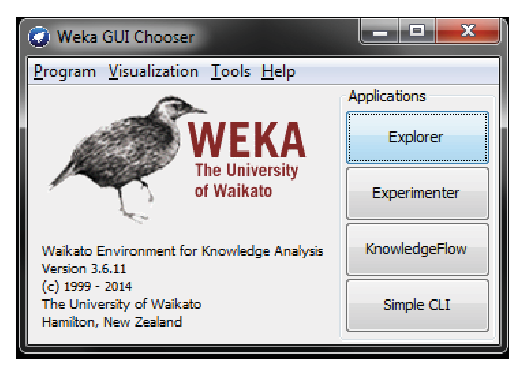
\includegraphics[scale=0.7]{figures/wekaGUI.eps}
  \caption{Weka GUI.}
  \label{fig:wekaGUI}
  \end{center}
\end{figure}

Next you should select the Explorer button
and Weka Explorer will be launched as depicted in Fig. \ref{fig:wekaExplorer}. Select the open file 
button in Weka Explorer and choose the the data set to be tested.

\begin{figure}[htb]
  \begin{center}
  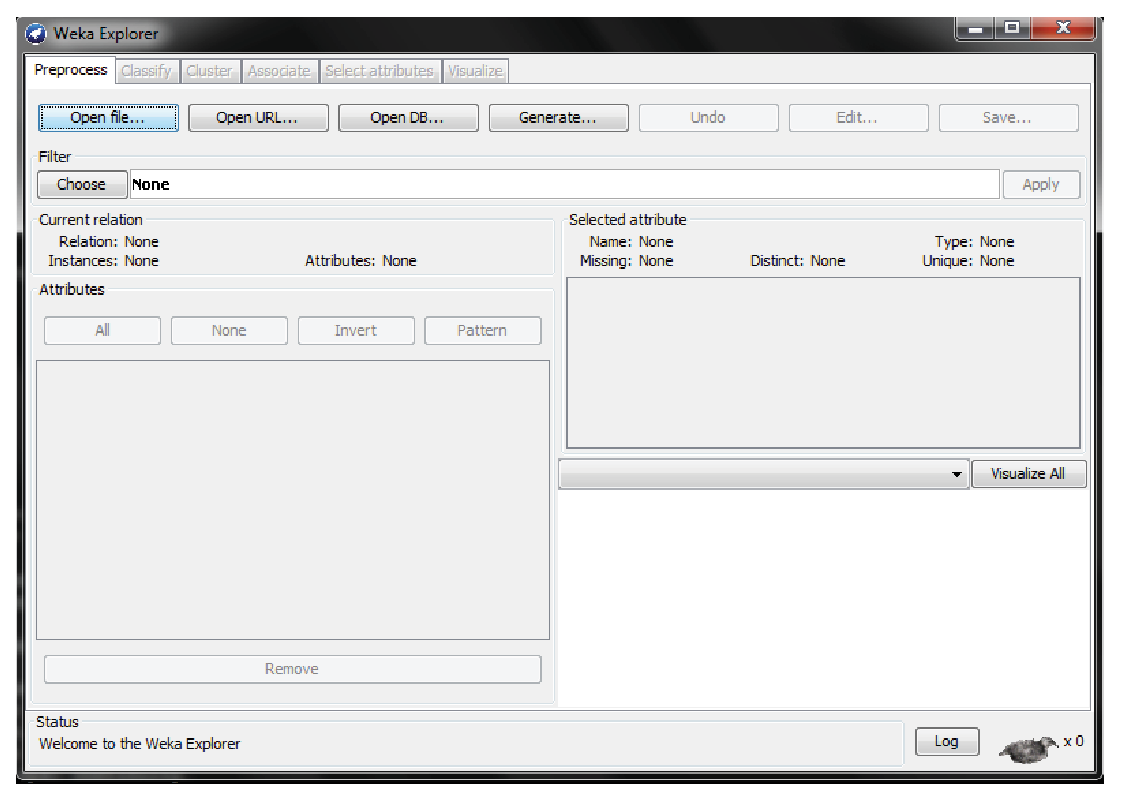
\includegraphics[scale=0.5]{figures/wekaExplorer.eps}
  \caption{Weka Explorer.}
  \label{fig:wekaExplorer}
  \end{center}
\end{figure}

Next choose the Classify menu in Weka Explorer and you will see the available classifiers as depicted 
in Fig. \ref{fig:wekaClassifiers}. You will find EAR4 under lazy classifiers category. 

\begin{figure}[htb]
  \begin{center}
  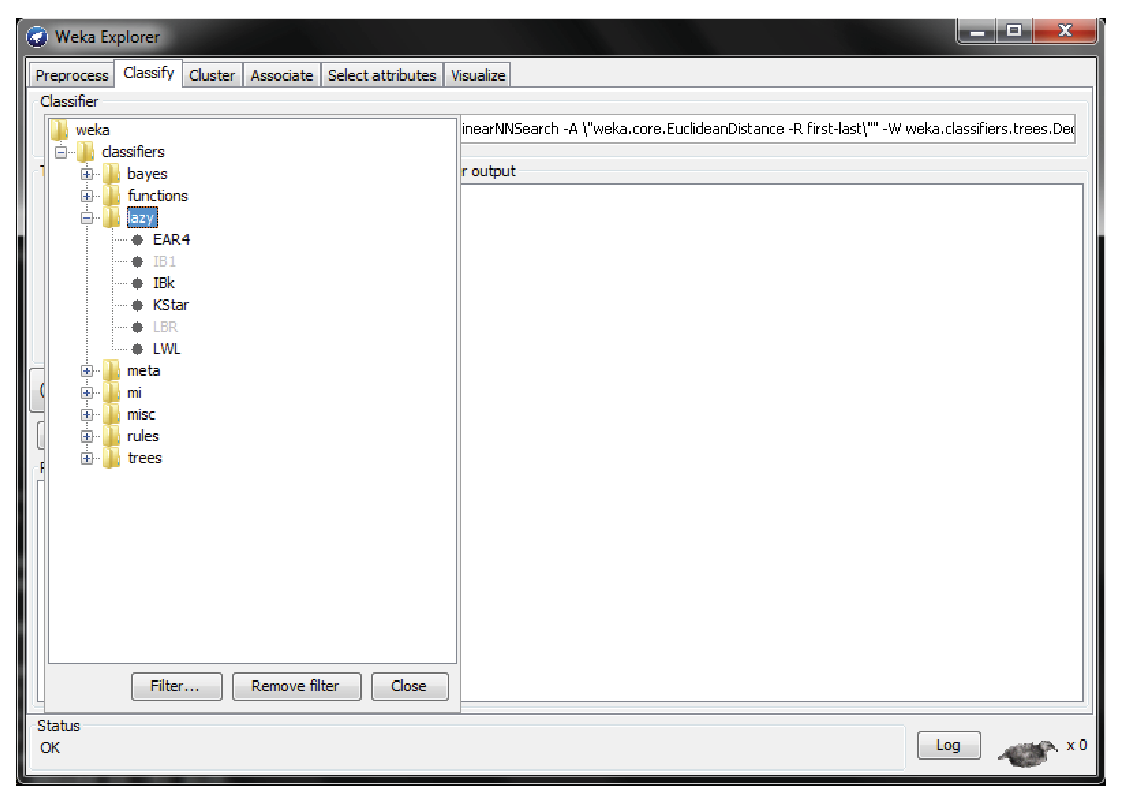
\includegraphics[scale=0.4]{figures/wekaClassifiers.eps}
  \caption{Weka Classifiers.}
  \label{fig:wekaClassifiers}
  \end{center}
\end{figure}


Choose EAR4 as the classifier.
Now you can tune the parameters used by EAR4 by clicking on the text box next to the choose button 
as depicted in Fig \ref{fig:ear4Parameters}.

\begin{figure}[htb]
  \begin{center}
  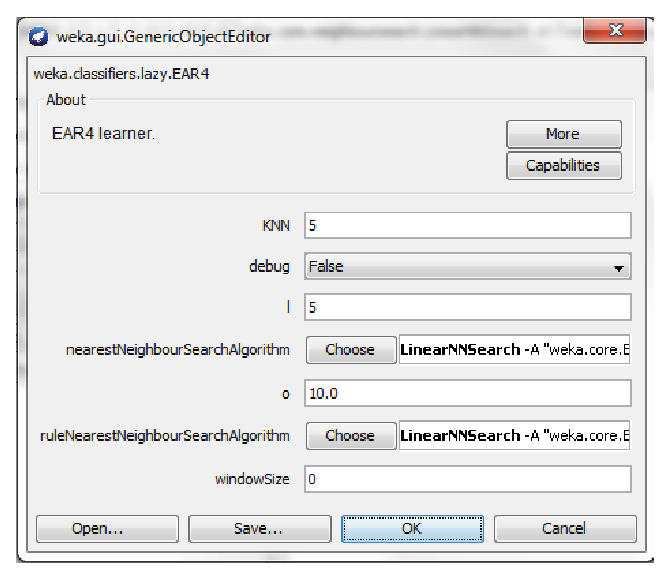
\includegraphics[scale=0.5]{figures/ear4Parameters.eps}
  \caption{Setting EAR4's parameters.}
  \label{fig:ear4Parameters}
  \end{center}
\end{figure}


As you can see in Fig \ref{fig:ear4Parameters} you can tune different parameters for EAR4. $kNN$ 
specifies the number of nearest neighbors that should be used in estimating the solution.
$l$ denotes the number of adaptation rules to be applied for adjusting the value of each neareset neighbor (base case).
$o$ is a coefficient used for determining the neighborhood used for adaptation generation. 
EAR4 generates adaptations based on the local neighborhood of the input query.
$o$ is a coefficient used for determining the number of nearest neighbors of 
the input query from which the adaptations should be generated. The number of
nearest neighbors of the input query from which adaptations are generated is derived by 
multiplying $kNN$ and $o$. The default value of $o$ is one, which means by defualt
the adaptation rules are built based on the the top $kNN$ nearest neighbors (i.e. base cases) of the input query. 
However, it makes sense to use values greater than one for $o$ in practice to make EAR4 more 
flexibile. $nearestNeighbourSearchAlgorithm$ and $ruleNearestNeighbourSearchAlgorithm$ also show the similarity measures 
used for retrieving the base cases and the adaptations respectively.
Figure \ref{fig:ear4Parameters} shows a sample valuations of EAR4 parameters. 

In this case, EAR4 estimates the input query's value by combining the adjusted 
values of the five nearest neighbors of the input query. While the
value of each of those nearest neighbors is adjusted by applying five adaptation rules. 
The adaptation rules are built from the top 50 (i.e. $5 \times 10$) cases of the input 
query.

Optimal values of EAR4's parameters can be tuned by hill climbing on the training data using 
cross validation. However, this feature is not currently implemented and 
it is up to the user to find and set the optimal tuining for the learner in practice.
 
%%%%%%%%%%%%%%%%%%%%%%%%%%%%%%%%%%%
%
%   This program is free software: you can redistribute it and/or modify
%   it under the terms of the GNU General Public License as published by
%   the Free Software Foundation, either version 3 of the License, or
%   (at your option) any later version.
%
%   This program is distributed in the hope that it will be useful,
%   but WITHOUT ANY WARRANTY; without even the implied warranty of
%   MERCHANTABILITY or FITNESS FOR A PARTICULAR PURPOSE.  See the
%   GNU General Public License for more details.
%
%   You should have received a copy of the GNU General Public License
%   along with this program.  If not, see <http://www.gnu.org/licenses/>.
%

% Version: $Revision: 8032 $

\begin{thebibliography}{999}
	% to make the bibliography appear in the TOC
	\addcontentsline{toc}{chapter}{Bibliography}

	\bibitem{jalali-Leake13-2}
	Jalali, V., Leake, D.:
	\newblock Extending case adaptation with automatically-generated ensembles of
	  adaptation rules.
	\newblock In: Case-Based Reasoning Research and Development, \uppercase{ICCBR}
	  2013, Berlin, Springer (2013)  188--202

	\bibitem{mantaras-et-al05}
	{Lopez de Mantaras}, R.; McSherry, D.; Bridge, D.; Leake, D.; Smyth,
	  B.; Craw, S.; Faltings, B.; Maher, M.; Cox, M.; Forbus, K.; Keane, M.;
	  Aamodt, A.; and Watson, I.
	\newblock 2005.
	\newblock Retrieval, reuse, revision, and retention in \uppercase{CBR}.
	\newblock {\em Knowledge Engineering Review} 20(3).

	\bibitem{aha91}
	Aha, D., Kibler, D.:
	\newblock Instance-based learning algorithms
	\newblock Machine Learning (1991) 37--66

	\bibitem{hanney-keane97}
	Hanney, K., Keane, M.:
	\newblock The adaptation knowledge bottleneck: How to ease it by learning from
	  cases.
	\newblock In: Proceedings of the Second International Conference on Case-Based
	  Reasoning, Berlin, Springer Verlag (1997)  359--370

\end{thebibliography}


\end{document}
